%%%%%%%%%%%%%%%%%%%%%%%%%%%%%%%%%%%%
% KTHEEtitlepage_ex.tex
%
% Example of how to use the KTHEEtitlepage package.
% 
% Mats Bengtsson,  7/8 2006
%%%%%%%%%%%%%%%%%%%%%%%%%%%%%%%%%%%%
\documentclass[12pt,a4paper]{article}

\usepackage{filecontents,lipsum}
\usepackage[noadjust]{cite}
\usepackage{graphicx,wrapfig,lipsum}
\usepackage{wrapfig}
\usepackage[nonumberlist,acronym,shortcuts]{glossaries}
\graphicspath{{Images/}}

\usepackage{textcomp,xspace}
\newcommand\la{\textlangle\xspace}
\newcommand\ra{\textrangle\xspace}
\usepackage[T1]{fontenc}
\usepackage{lmodern}


\usepackage{listings,lstautogobble}
\usepackage{color}
\definecolor{dkgreen}{rgb}{0,0.6,0}
\definecolor{gray}{rgb}{0.5,0.5,0.5}
\definecolor{mauve}{rgb}{0.58,0,0.82}
%\lstset{escapeinside={<@}{@>}}
\lstset{frame=tb,
    %language=Java,
    aboveskip=3mm,
    belowskip=3mm,
    showstringspaces=false,
    columns=flexible,
    basicstyle={\small\ttfamily},
    numbers=none,
    numberstyle=\tiny\color{gray},
    keywordstyle=\color{blue},
    commentstyle=\color{dkgreen},
    stringstyle=\color{mauve},
    breaklines=true,
    breakatwhitespace=true,
    tabsize=3,
    escapeinside={<@}{@>},
    autogobble=true
}

\usepackage[exjobb]{KTHEEtitlepage}
%\renewcommand{\cftsecleader}{\cftdotfill{\cftdotsep}}

% Packages used in the main document for this particular example:
\usepackage{url}
\usepackage{tocloft}
\renewcommand\listfigurename{List of Figures}
\renewcommand\listtablename{List of Tables}


\newcommand{\quotes}[1]{``#1''}
\usepackage{hyperref}
%\usepackage{acro}
\hypersetup{%
	pdfborder = {0 0 0}
}
\usepackage[exjobb]{KTHEEtitlepage}

 \newacronym{asip}{ASIP}{Application Specific Instruction-set Processors}
 \newacronym{ebnf}{EBNF}{Extended Backus Naur Form}
 \newacronym{cpri}{CPRI}{Common Public Radio Interface}
 \newacronym{osi}{OSI}{Open Systems Interconnect model}
 \newacronym{gpp}{GPP}{General Purpose Processor}
 \newacronym{asic}{ASIC}{Application Specific Integrated Circuit}
 \newacronym{tlm}{TLM}{Transaction Level Modeling}
 \newacronym{pla}{PLA}{Programmable Logic Array}
 \newacronym{fpga}{FPGA}{Field Programmable Gate Arrays}
 \newacronym{rbs}{RBS}{Radio Base Station}
 \newacronym{ieee}{IEEE}{Institute of Electrical and Electronics Engineers}
 
 
 
 
 
 

\makeglossaries

\begin{document}
% Information to appear on the title page:
\ititle{Reconfigurable hardware programming in a protocol processor unit}
\isubtitle{}
\iauthor{- Sunil Kallur Ramegowda}
\idate{2015}
\irefnr{IR-EE-Dummy 2000:099}

\iaddress{ICT Labs\\
	Major in Embedded Platforms\\
		Kungliga Tekniska H�gskolan}
		\makeititle

		% Everything below is exactly as for a normal document and 
		% the layout of that document should not be affected in any
		% way by the title page.

		\title{Reconfigurable hardware programming in a protocol processor unit}
		\author{Sunil Kallur Ramegowda}

		\maketitle
		\pagenumbering{roman}
       
  		\begin{abstract}
		
        Reconfigurable hardware architectures are the topic of research for many years.Programming such architectures requires the design of custom compilers to generate the required files for the architecture.
        
        A protocol processor,in general processes the packets according to the protocol.There are number of protocols like Ethernet,\acs{cpri} to define how the data has to be sent and received between the source and destination points. Data packets can be processed using the generic processors programmed in software,but hardware processing is always energy efficient.\\  
        
        A compiler/mapper is developed in this thesis work. The language application was developed using a parser generator tool called Antlr.The grammar was written in \acs{ebnf} and the corresponding language was used to describe the architecture and the protocols. The tool will generate the hardware model and their interconnection in SystemC based on the protocol description.\\ 
        
        The complete system was verified by integrating the Ethernet protocol.Parts of the protocol implementation in SystemC was also considered in the work.The system is verified for different protocols.The framework works based on the user defined description of the protocol. \\
        
        Future work involves the integration of further protocols into the system and then adapt the language to further involve all the future requirements.The concept of mapping can be used to design the hardware blocks and their interconnections in different languages. 
        
        
		\end{abstract}
        \phantomsection
        
		\addcontentsline{toc}{section}{Abstract}
       	\cleardoublepage

        %\renewcommand\contentsname{\centerline{\underline{\underline{Table of Contents}}}}
		\phantomsection
        %\cleardoublepage
        %\addtocontents{toc}{~\hfill\textbf{Page}\par}
        \tableofcontents
        %\cleardoublepage
		\addcontentsline{toc}{section}{\contentsname}
		\cleardoublepage
        
        % abbreviations
        \phantomsection
        \addcontentsline{toc}{section}{Abbreviations}
        \printglossary[type=\acronymtype,title=Abbreviations]
        \cleardoublepage

		\phantomsection
		\listoffigures
		\addcontentsline{toc}{section}{List of Figures}
		\cleardoublepage

		\phantomsection
        \listoftables
		\addcontentsline{toc}{section}{List of Tables}
		\clearpage

		\pagenumbering{arabic}
         
       \section{Introduction}

		A set of digital rules define the communication strategy between digital systems.There are many rules which makes the communication possible between systems.Over the decades the rules have evolved into standards.The rules are called as Protocols in communication systems.The \gls{osi} partition the communication system into 7 abstraction layers.There are different protocols for each layers of abstraction. The software and/or hardware changes based on the protocol chosen to process the message and extract the relevant information at each layer of abstraction. The hardware solutions based on a \gls{gpp}  or an \gls{asic} exists \cite{5335678}\cite{558379}.GPP will have more flexibility but are less energy efficient when compared to \acs{asic} which are less flexible and most energy efficient. \acs{asip} or domain specific processors are more suitable for the protocol processing task and depending on their architectural characteristics they allow varying degrees of trade-off between flexibility and energy-efficiency\cite{1106752}.Resource and performance varies depending on the reconfigurable architecture and its level of abstraction\cite{6868627}.\\   

		The design of reconfigurable hardware architecture requires the compiler to produce the configuration or the hardware compatible code.These files can be produced on run time when the application is running or in a static way before the application is made to run. The complexity of the system depends on the selected design.The hardware for processing the different protocols can be made reconfigurable.Investigation and design of such a concept is performed in this thesis work.\\ 

		The reconfigurable hardware is modeled in SystemC language using \acs{tlm}. The configuration files required for the reconfiguration is obtained by parsing the description of protocols using the language defined by the Grammar.The Antlr tool is used for building the base parser file for the defined grammar and then the required functions are written to output the complete system and configuration files. 
        

		\clearpage
		\subsection{Background}
		In 1960 Gerald Estrin, proposed the idea of a fixed plus variable structure computer \cite{1114865}.It consisted of a fixed processor and an array of reconfigurable hardware which was controlled by the fixed processor.Even though the idea was demonstrated with a proof,the industry did not consider to further innovate in these field and till 1980's there were no significant developments. In  1985,the reconfigurable \gls{pla} was patented\cite{page1985re}.Innovation in \acs{pla}'s further continued with the commercially available \gls{fpga} in today's market.\\

		Ericsson AB is a market leader in the radio base station equipments.There are different protocols being used for communication in the Radio Base Station (RBS) units.Ethernet standard explained by \acs{ieee} in 802.3 standard defines the protocol for 10Gbit transfer which is mainly used for communication between the silicon chips. Other protocols include \gls{cpri},Serial Rapid IO(SRIO),Xio(Ericsson Specific protocol) for reliable communication between chips at high data rate.Most of these protocols in MAC layer of abstraction have common hardware units. Ericsson design and manufacture Custom \acs{asic} chips for these protocols.The common functions which can be used by different protocols for designing a reconfigurable hardware architecture which will minimize the cost and will provide more flexibility compared to ASIC chips.More details about the protocols and reconfigurable architecture is explained in Chapter 3.\\ 

		The reconfigurable architecture requires a new hardware and software co-design.The reconfiguration details are extracted based on the hardware design and the compiler/mapper should be able to produce such reconfiguration.This is accomplished  by using Grammar based technique i.e by defining a language based on \gls{ebnf} grammar and then describing the protocols using this language.The overall architecture and working principle will be explained in further chapters.\\

		The thesis deals with understanding the reconfigurable architecture and identifying the configuration details to make the system work for different protocols.The description in high level language is used to extract these configuration details and to verify the complete system using a test bench.\\   

		\clearpage


		\subsection{Purpose}

		The thesis purpose is to investigate an approach of a compiler or mapper to describe the protocols in high level language and then map it to hardware blocks and their interconnection.This involves showing the proof of concept by SystemC TLM simulation models.The Individual hardware blocks are modeled in SystemC and can vary from a simple block to complex functions of the protocols like Encoder.This thesis work serves as a proof for the project in Ericsson AB to further investigate the feasibility of developing such architectures.



		\subsection{Goals}
		The thesis goal is to achieve the below milestones:
        
        \begin{itemize}
            \item{Understand the Reconfigurable hardware architecture designed at Ericsson AB}
            \item{Understand Ethernet,Xio and CPRI protocols}
            \item{Define a language to describe the protocols in high level words}
            \item{Identifying how to represent the reconfiguration information}
            \item{Mapping the description of language to hardware and interconnections}
            \item{Integrating Ethernet protocol for the complete system}
            \item{Verifying the system by simulation}
            
            
        \end{itemize}
        
      	               

		\subsection{Limits on scope}
		The thesis focus more on showing the proof of concept considering one to two protocol i.e Ethernet and Xio. The language will be designed such that it is easy with minor modification to extend for other protocols like CPRI,SRIO. Developing and integrating the \acs{tlm} models for all the protocol's will not be feasible in this time line.

		\subsection{Structure of the thesis}
		The thesis is organized to provide required details for understanding the overall work. The first chapter gives a brief introduction to the reader about the topic of investigation,limitations and goals.The second chapter will describe the background about the topic and the literature about different terminologies. The third Chapter will provide the implementation details and the results obtained will be explained in chapter four. The Future work and conclusion are stated in the further chapter five  and six.


		\clearpage


		\section{Background}
		To understand the reconfigurable hardware and its terminologies, this chapter explains in detail about the architecture and its meaning.Protocols and their common functions are also explained which helps in designing the reconfigurable protocol processors.The further sections explains the meaning of grammar and language and its terms.    


		\subsection{Reconfigurable Systems}


		In the field of computer architecture, designers make decisions based on flexibility and performance requirement\cite{JACST518}.\acs{asic} are the least flexible in terms of adapting for any change in the application and GPP are the most flexible as they are independent of the application and the core can be programmed to make the required algorithm work at the cost of higher power and lower efficiency.ASIC and GPP lies in extreme corners of the graph between Flexibility Vs Performance as in Fig.~\ref{fig:Fig1}.Reconfigurable architectures are intended to fill the gap and provide more flexibility in terms of hardware and potentially higher performance than software\cite{JACST518}.

		\begin{figure}[!htb]
		\centering
		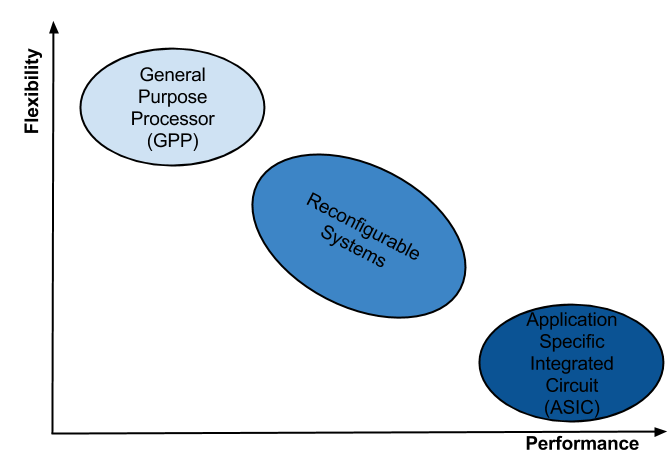
\includegraphics[scale=0.45]{Fig1}
		\caption{Flexibility Vs Performance of Hardware Classes}
		\label{fig:Fig1}
		\end{figure}

		\subsubsection{Granularity}

		Reconfigurable devices like \acs{fpga} have the configurable logic blocks(CLB) which can be configured to map the required functionality. The complexity of the function is not a concern but the number of inputs and output of the function has to be considered based on the FPGA architecture. This level of granularity in implementing the functions is called as Fine grained Reconfigurable architecture as it provides the reconfigurable granularity till lowest possible level. These reconfigurable devices are not energy efficient and the execution speed is too less than the ASIC counterpart. Another type of reconfigurable devices are the coarse grained reconfigurable architectures. These devices have the granularity at function levels. They will configure the Function blocks to achieve the efficient algorithm implementation.The Function blocks can vary from constant blocks to complex functions which are commonly used based on the application domain.   


		\subsubsection{Reconfiguration Models}
		The reconfigurable architectures need configuration of hardware.This can be at compile time or at runtime of an application as in  Fig.~\ref{fig:Fig2}.

		\begin{figure}[!htb]
		\centering
		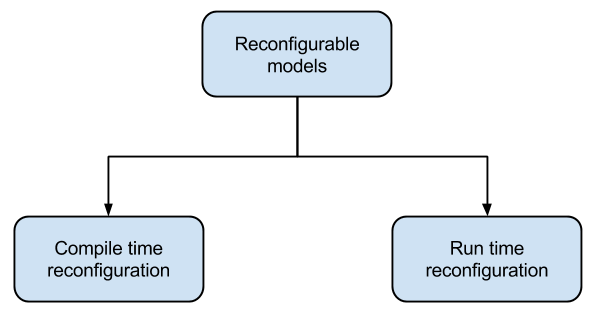
\includegraphics[scale=0.45]{Fig2}
		\caption{Reconfiguration Models}
		\label{fig:Fig2}
		\end{figure}

		In Compile time reconfiguration model, the reconfigurable hardware system is configured at compile time and will be static during the application run time.In this model the programmable logic can be configured to perform some specific task like hardware accelerators to achieve high performance.FPGA configured to perform floating point multiplication together with a GPP will accelerate the performance of the application if the GPP doesn't have a Floating Point Unit.
		In Run time reconfiguration model, the reconfiguration hardware is configured at run time and will be dynamically programmed to perform different tasks.The decision for making such dynamic reconfiguration has to be embedded coupled with the application and hence it increase the overhead.The Dynamic Reprogrammable Resource Array(DRRA) fabric developed at KTH Electronic System Dept is an example of this model\cite{5351593}.   

		\subsubsection{Reconfiguration rate}
		The Fine grain Systems will have more reconfiguration data(In FPGAs it is in term of bit streams) which leads to more time and the Coarse Grained Reconfigurable systems will have comparatively less blocks as they have higher granularity and will contain less reconfiguration data.Hence the Coarse Grain architecture will take less time to re configure. This depends on the dynamic reconfiguration architecture whether the complete fabric is reconfigured or partially reconfigured during runtime. 


		\subsection{Protocols}

		The communication between chips in Radio Base station equipments has many protocols to fulfill the requirements of the specification.The protocols differ by standards.The Data link layer protocol's of the \acs{osi} model share some common functionalities.The different protocols being used at Ericsson AB and related to this thesis work are described below:  

		\subsubsection{Ethernet}
		Ethernet is a widely used protocol for data communication. It is typically used in Local Area Network (LAN) applications. IEEE organization has standardized the protocol and revises it according to the technological advancement. The recent standard available is from 2012 and it defines the protocol for different applications.
        
        \subsubsection*{Ethernet Transmit}
            The Ethernet transmit sequence is shown in Fig.~\ref{fig:EthTx}.
        
       \begin{figure}[!htb]
            \centering
            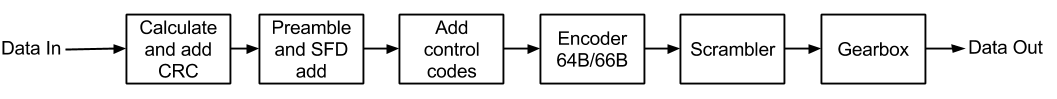
\includegraphics[scale=0.45]{EthTx}
            \caption{Ethernet Transmit}
            \label{fig:EthTx}
       \end{figure}
       
       The \textit{DataIn} is from the Job description tokens which contains the data to be transmitted using MAC layer protocol.Physical layer protocols are out of this thesis scope and not explained.
       
        
       \subsubsection*{Ethernet Receive}
           The Ethernet Receive sequence is shown in Fig.~\ref{fig:EthRx}. \textit{DataIn } is from the Physical transmission layer and \textit{Dataout} is to the higher protocol layers.
       
            \begin{figure}[!htb]
             \centering
             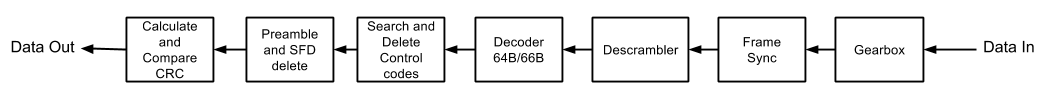
\includegraphics[scale=0.45]{EthRx}
             \caption{Ethernet Receive}
             \label{fig:EthRx}
            \end{figure}
            
       \subsubsection*{Ethernet Raw frame}
       
       The Ethernet raw frame format is represented as in Fig.~\ref{fig:ethframe}.Each of these frames enter the transmitter as Datain as in
       Fig.~\ref{fig:EthTx} and in the receiver as Data out as shown in Fig.~\ref{fig:EthRx}. 
       
        \begin{figure}[!htb]
            \centering
            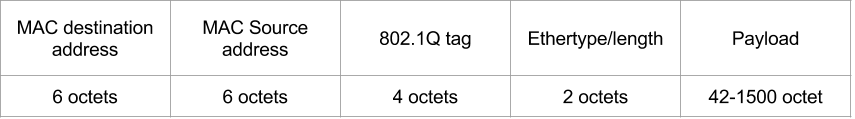
\includegraphics[scale=0.45]{ethframe}
            \caption{Ethernet Raw Frame}
            \label{fig:ethframe}
            \end{figure}
        
       A brief functional description of each blocks in the transmitter and receiver section is explained below.
       
       \subsubsection*{CRC}
        Cyclic Redundancy check is used to detect errors incurred during the physical transmission. The CRC value is computed by dividing the data to be transmitted with the pre-defined CRC polynomial stored in the memory\cite{4066263}. The remainder of the division is known as the Frame Check Sequence (FCS).\\ 
        
        In transmitter side the FCS is computed for the incoming data and appended as last 4 bytes (32bits). In the Ethernet receive, the FCS is again computed for the incoming data and is compared with the FCS field for any errors.  This block will not change the incoming data apart from appending the FCS field at the end.
        
        \subsubsection*{Preamble and SFD}
        Preamble is added at the start of the frame to indicate the new Ethernet frame. This block will not change the incoming data apart from adding the Preamble(7bytes) and Start of Frame Delimiter (SFD) at the beginning of the frame(1byte).\\ \\
        Preamble:  Total 7bytes, each byte is 10101010.\\
        SFD: 10101011 \\
        
        In the receiver, the Preamble and SFD are identified and deleted.
        
        \subsubsection*{Control codes}
        
        The Add control codes block will add the control codes for the incoming data such that Encoder block can use the 8 octets to encode the data based on this control codes. Idles are added to the data if the length of the data is not equal to 8 octets. Each bit in the control word represents whether the octet is data, terminate or an idle octet.
        
        \begin{figure}[!htb]
            \centering
            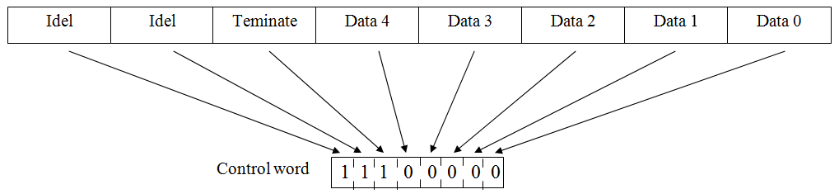
\includegraphics[scale=0.45]{controlword}
            \caption{Control Word}
            \label{fig:controlword}
        \end{figure}
        
        In the receiver, the complete process is reversed. It will search for the control word and delete before forwarding to the next block.
        
         \subsubsection*{Encoder 64/66B and Decoder 66B/64B}
         
         The Encoder block is represented as show in Fig.~\ref{fig:encoder}. The 8 octet data is encoded using the control word into 66 bit output. The first 2 bits of the output are called sync header which is used for the synchronization from the receiver. The synch header \quotes{10} correspond to data and \quotes{01} corresponds to control codes
         
          \begin{figure}[!htb]
              \centering
              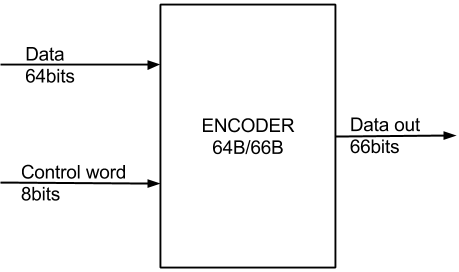
\includegraphics[scale=0.45]{encoder}
              \caption{Ethernet Encoder block}
              \label{fig:encoder}
            \end{figure}
        
        In the decoder the synch header is used to synchronize the 66bit data. The process of decoder is the reverse interpretation of the encoder module.
        
        \begin{figure}[!htb]
            \centering
            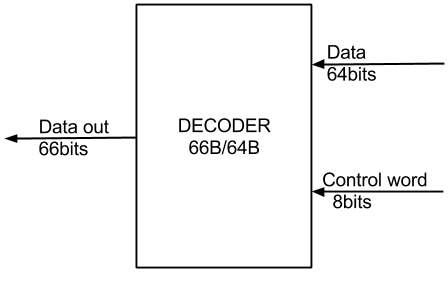
\includegraphics[scale=0.45]{decoder}
            \caption{Ethernet Decoder block}
            \label{fig:decoder}
        \end{figure}
        
        
         \subsubsection*{Scrambler and Descrambler}
            
            This block is used to randomize the signal so that long sequence of 1?s and 0?s are eliminated. This is performed using the Scrambler polynomial.
            
            The Descrambler will take the scrambled input and will output the unscrambled data.  
        
         \subsubsection*{Gearbox}

           This block is used to switch between different output rates. The incoming data is transmitted at different rates based on the clock frequency.
           

        
        
		\subsubsection{Xio-s}
		Xio-s is Ericsson proprietary protocol used for communication between chips.
        
        \begin{figure}[!htb]
            \centering
            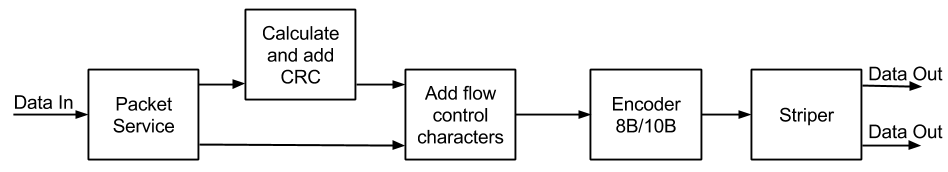
\includegraphics[scale=0.45]{Xiotx}
            \caption{Xio-s Transmitter}
            \label{fig:Xiotx}
        \end{figure}
        
        
        \begin{figure}[!htb]
            \centering
            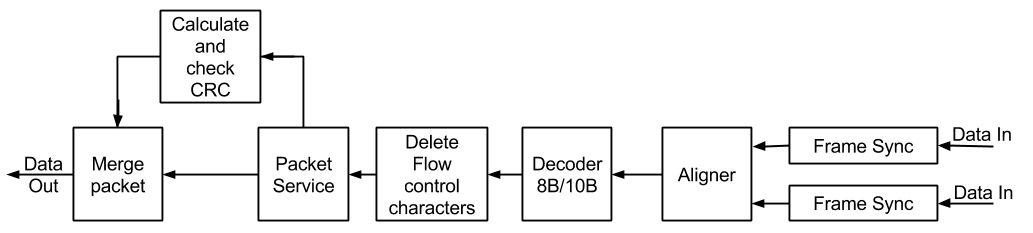
\includegraphics[scale=0.45]{XioRx}
            \caption{Xio-s Receiver}
            \label{fig:XioRx}
        \end{figure}
        
        \begin{figure}[!htb]
            \centering
            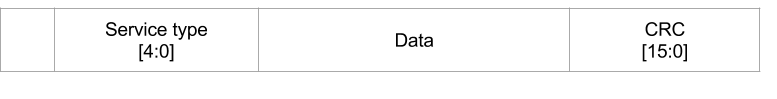
\includegraphics[scale=0.45]{xiotype1}
            \caption{Xio-s Frame format Type 1}
            \label{fig:xiotype1}
        \end{figure}
        
        \begin{figure}[!htb]
            \centering
            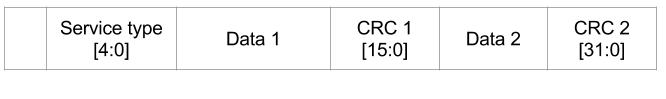
\includegraphics[scale=0.45]{xiotype2}
            \caption{Xio-s Frame format Type 2}
            \label{fig:xiotype2}
        \end{figure}
        
        There are 7 different types of packet services for Xio-s protocol. This assigns the packet to proper channel based on the service type. As an example, if the service type format 1 then it uses only CRC16 channel or if the Service type format II then it uses both CRC16 and CRC32 channels.
        
        
        \subsubsection*{CRC}
        There are 16bit and 32bit CRC calculations required in Xio-s protocol. So the polynomials for CRC16 and CRC32 are stored in the memory and the function is used according to the service type.
        
        In the receiver, the CRC is again computed and compared with the received bytes. 
        
        
        \subsubsection*{Flow control characters}
        
        The flow control character will add the control word similar to Ethernet protocol in each channel. These are used for indication of start and end of frames.
        
        In the receiver the flow and control characters are identified and deleted.
        
        
        \subsubsection*{Encoder/Decoder}
        The encoder module will encode one octet at a time to 10bits.So for 8 octects it outputs 80bits The encoder 8B/10B is invented by IBM and famous for short run length and DC balance.
        
        The decoder module does the reverse of encoder and thus the output of decoder will be the same as the input of encoder.
        
        \subsubsection*{Striper}
        It is used to split the 80bits incoming data into 40bits of 2 physical channels to increase the data transfer rate.
        
        
        \subsubsection*{Frame Sync}
        This block is used to synchronize the receiving data.It is performed using the special character in the transmitted data called as k28.5 character.
        
        
        \subsubsection*{Aligner}
        This block is used in the receiver if striper is used in the transmitter side.It aligns the two incoming 40bits channels into one 80bits channel.
        
        
		\subsubsection{CPRI}
		
        
        
         \begin{figure}[!htb]
             \centering
             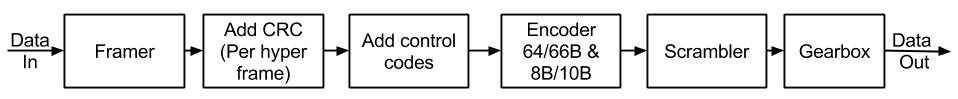
\includegraphics[scale=0.45]{cpritx}
             \caption{CPRI Transmitter}
             \label{fig:cpritx}
            \end{figure}
            
         \acs{cpri} is an industry cooperation aimed at defining a publicly available specification for the key internal interface of radio base stations between Radio Equipment Control(REC) and the Radio Equipment(RE).It is the co operating work of Ericsson AB,Huawei Technologies Co.Ltd,NEC corporation,Nortel Networks SA and Siemens AG.   
         All the blocks in this protocol are similar to the blocks in Ethernet protocol. The frame structure is similar to the Xio-s protocol.
         
            
            
        \begin{figure}[!htb]
            \centering
            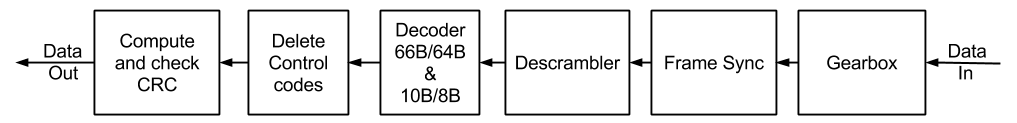
\includegraphics[scale=0.45]{cprirx}
            \caption{CPRI Receiver}
            \label{fig:cprirx}
        \end{figure}
        
        
        
        \subsubsection{Comparison of 3 Protocols}
            
           The common functions in each protocol are highlighted with the same color for the boundary line in Fig \& Fig. A common hardware architecture can be designed with minimal reconfiguration to perform the protocol processing of different protocols stated above.\\
        
        
        
         \begin{figure}[!htb]
             \centering
             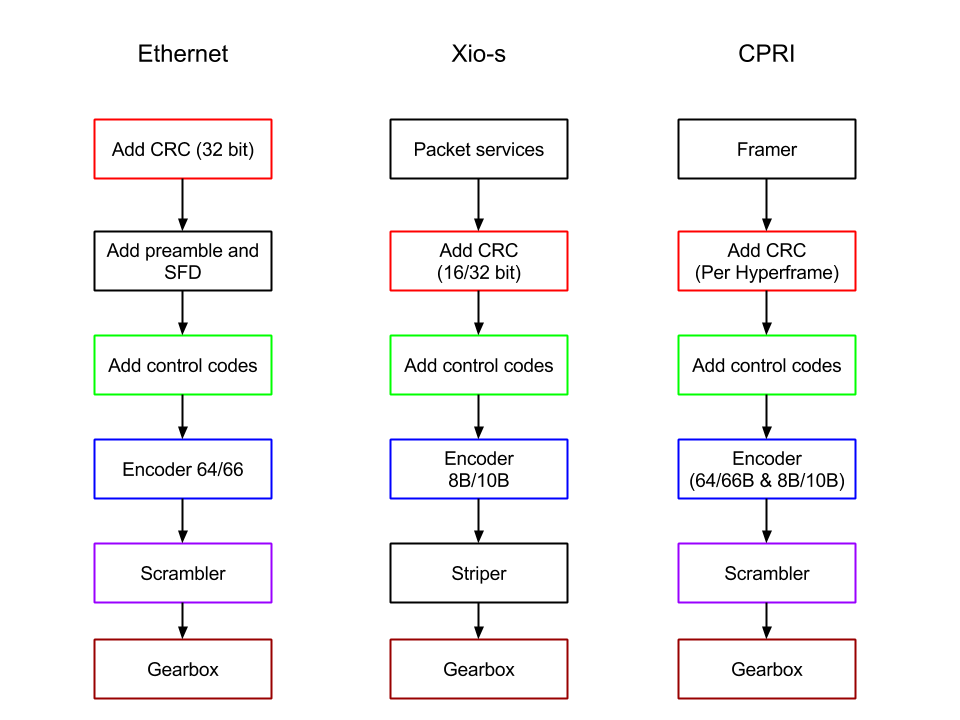
\includegraphics[scale=0.4]{common_tx}
             \caption{Transmitter of all 3 protocols}
             \label{fig:common_tx}
            \end{figure}
        \clearpage

         \begin{figure}[!htb]
             \centering
             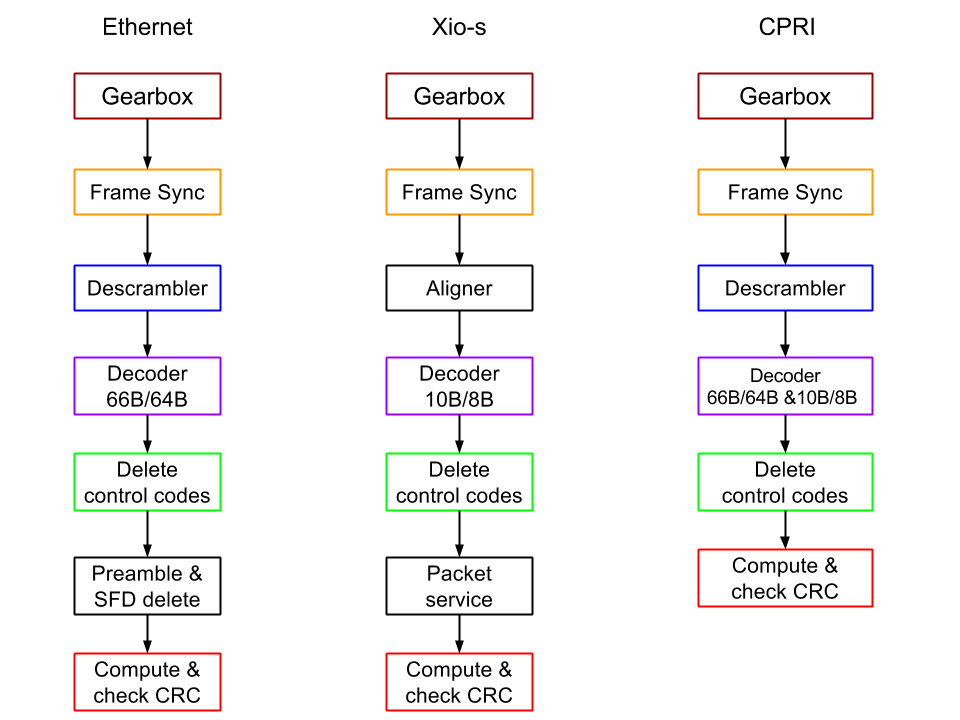
\includegraphics[scale=0.4]{common_rx}
             \caption{Receiver of all 3 protocols}
             \label{fig:common_rx}
            \end{figure}

        \clearpage
        
        
        
        

	    \subsection{Grammar and Language}
        
        A Grammar is used to describe the syntax of a language, that is, all possible legal sentences or combination of words that make up the language. More formally, Grammar G describes all allowed legal sequences of strings. This is called the language(G) of the grammar.
        The language in turn is made of sequence of elements which can be letters, numbers or special symbols. For example, In the word \quotes{KTH} the capital letters K,T,H are to be recognized and then the word needs to be formed. This is performed by the Lexer which recognizes the letter and forms the token.
        To be able to recognize words, Lexer need some special constructs. These special constructs makeup the language that can be recognized by regular expressions. For example, regular expression [0-9] recognizes a single letter in the range from 0 to 9. 
        
        
        \subsubsection{Parser}
            The Lexer scans the input character streams and forms the valid tokens. The Parser takes tokens as inputs and then based on the parsing rules in the grammar, decides the parsing strategy. The parser output can be used either to create an interpreter or a compiler. 
            
            
            \begin{figure}[!htb]
                \centering
                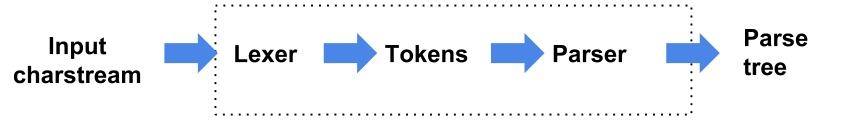
\includegraphics[scale=0.45]{parsetree}
                \caption{Parser}
                \label{fig:parsetree}
            \end{figure}
        
        
        Here,a language application is built to output the reconfigurable hardware architecture.Hence the parser output is used to translate it to the required output. 
        
        \subsubsection{Backus-Naur Form}

		In computer science world, BNF is the notational technique for context free grammars. It is a set of derivation rules to define the language.\\ 
        
        For example,\\
           
       \la int\ra  \hspace{0.2cm} ::= \la DIGIT \ra    | \la int \ra  \la DIGIT \ra \\
       
               \la DIGIT \ra \hspace{0.2cm} ::= [ 0-9 ]
        
        In the above Grammar, \la int \ra on the left hand side is called as non terminal and the \la DIGIT \ra is called as terminal. So the sequences of digits like 9999... can be parsed by representing grammar using BNF. 
        An extension to BNF grammar with more operators to write the syntax is called as EBNF. The grammar above can be rewritten in EBNF as below \\
        
        \la int \ra ::= \la DIGIT \ra * \\
        
        Here * means one or more occurrences of digits. Similarly \quotes{+} operator means 0 or more occurrences.
        
        

		\subsubsection{Antlr}

		ANTLR is a powerful parser generator that can be used to read,process or translate structured text or binary files.It has been adapted in academia and industries for different applications and hence there is a good community help for most common problems.The tool generates the background parser and checker files for the grammar defined in the Bacchus-Naur form(BNF)or the Extended Bacchus-Naur form(EBNF).It makes the framework easy for the user to generate a language application based on the defined grammar.
        
        
        \begin{figure}[!htb]
            \centering
            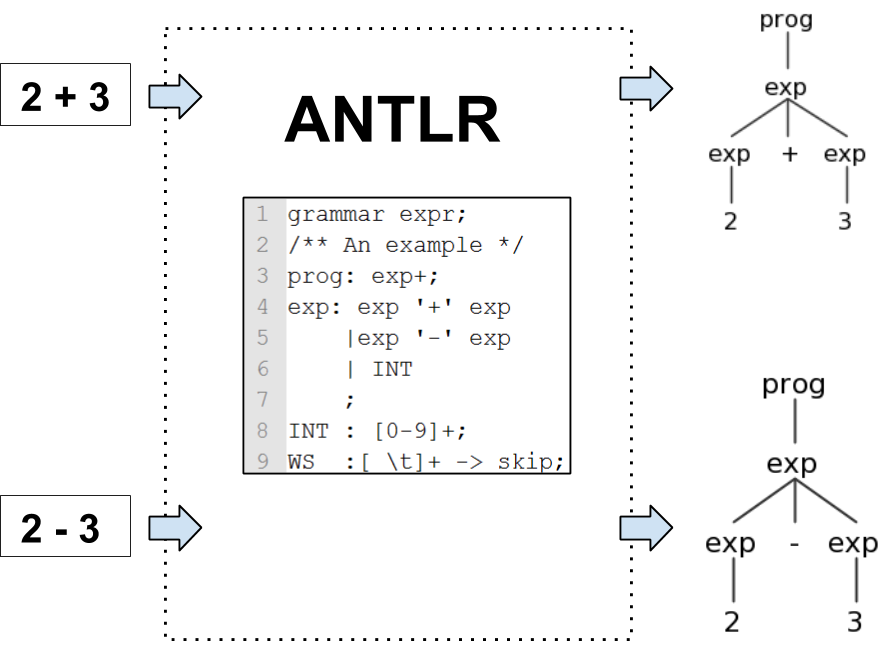
\includegraphics[scale=0.4]{antlr}
            \caption{Antlr}
            \label{fig:antlr}
        \end{figure}
        
        
        
        Antlr is a parser generator tool.It allows the user to express the grammar to match syntactic structures like programming language arithmetic expressions.As in Fig below, the grammar can parse the expression and produce the parse tree and the backend functions to implement the interpreter, compiler or translator .
        

        \subsubsection*{Parse tree listners and Visitors}
            Antlr provides 2 tree walking mechanisms in its runtime library. In parse tree Listners, ANTLR generates a parsetreeListner subclass specific to each grammar with entry and exit methods for each rule. This is suitable for applications wherin the complete tree need to be invoked from root till the last leaf node. The parse tree Visitor mechanism is used when the tree walking needs to be controlled.
        

		\clearpage
		\subsection{Environment and Tools}
        The Linux based server environment is used for compiling and testing the project files.The Antlr tool is used to define the protocols in a language defined in the grammar using EBNF. The Antlr tool is made to ouput the state table information which contains all the states with transition information.This will be used to reconfigure the hardware to process the input packets according to the protocols.
        
           
        \subsubsection{SystemC}
         SystemC is an ANSI standard C++ class library for system and hardware design for use by designers and architects who need to address complex
         systems that are a hybrid between hardware and software \cite{1617814}.It helps in modeling the concurrent processes.This makes it possible to model the hardware which are concurrent systems by nature.  
        
        \subsubsection{TLM}
         Transaction level Modeling is the approach of abstracting the lower implementation details of the function units and representing the overall system architecture.TLM helps in modeling the communication and the function unit implementation separately. The Transaction refers to the set of data being exchanged.TLM speeds up the simulation by replacing a set of pin level events with a single function call.\\
         
         TLM 2.0 standard is used for the implementation of the bus system.
         
       \subsubsection{UVM}
       Universal Verification Methodology(UVM) is a verification methodology based on the best features of OVM(Open verification Methodology) and Verification Methodology Manual(VMM).A Base version of UVM is built to verify the functionality of the architecture.  
       
		\clearpage


       \section{Methodology}
       
       This chapter starts with a description of the methodology behind the research process. The representation of test results, analysis and their methods are discussed. 
       
       \subsection{Research process}
            The architecture and its interconnections need to be understood to design the protocol processor. The reconfigurable architecture is called as Freyja architecture.
       
       
       \subsubsection{Freyja Architecture}
           As in Fig , Freyja architecture is a reconfigurable protocol processor. It consists of different protocol operators which are connected through the central switch. This switch based network topology can be configured to process the data based on protocols. The Ring bus (RB) interface the Freyja with the higher layers of protocol and it issues the data frames of different protocols as tokens. The Common Memory Interface(CMI) is used to fetch the data from memory. 
           The physical interface is represented by the Serializer/Deserializer block i.e SERDES. The details of each of the Freyja architecture blocks are discussed below.
           
            \begin{figure}[!htb]
                \centering
                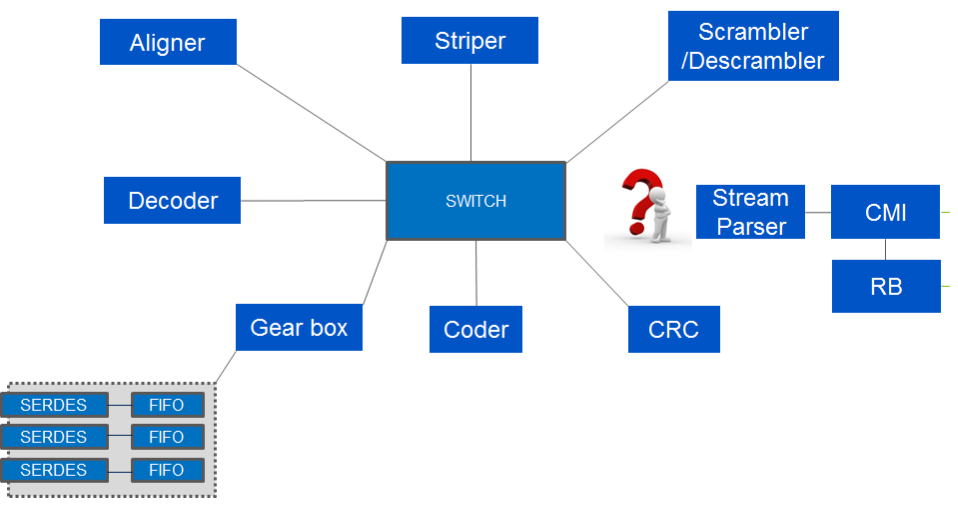
\includegraphics[scale=0.4]{Freyja}
                \caption{Freyja Architecture}
                \label{fig:Freyja}
            \end{figure}
           
       
       \subsubsection*{Switch port}
       
       \begin{wrapfigure}{R}{0.4\textwidth}
           \vspace{-30pt}
           \centering
               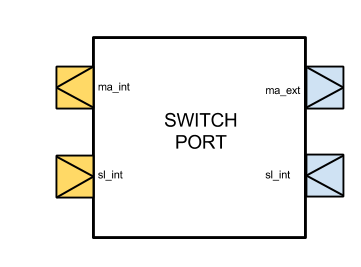
\includegraphics[width=0.4\textwidth]{switchport}
            
            \caption{Switch port}
            \label{wrap-fig:switchport}
            
        \end{wrapfigure} 
        
       Freyja Switch port is the smallest unit in the architecture which receives the transactions from different functions and then forwards it to the internally connected next switch port based on the destination of the transaction. It consists of a simple initiator socket,simple target socket,Multipass through initiator socket and Multi pass through target socket.It is represented as in \lipsum[0-0] Figure~\ref{wrap-fig:switchport}
       
       
       
       
       \subsubsection*{Operator units}
       
       
       \begin{figure}[!htb]
           \centering
           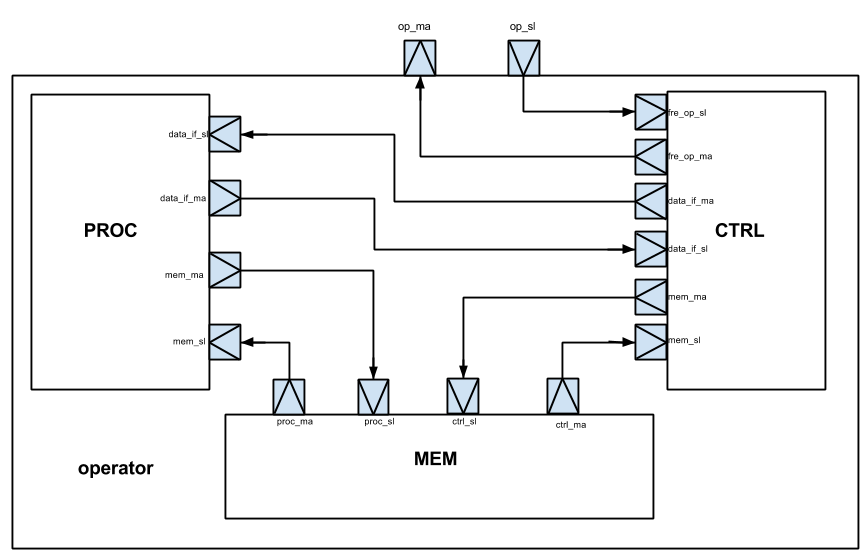
\includegraphics[scale=0.4]{operator}
           \caption{Freyja operator}
           \label{fig:operator}
        \end{figure}
       
      
       Freyja Operator units are designed to contain a control, process and memory blocks. Each operator function is implemented in the process block and the transaction routing and context switching is performed in the control block. The memory block stores the constants required for the process block. It can also be used to store the result and then the control block can access the results. 
       As in Fig , the 3 components of each operator is encapsulated with one simple initiator socket and one target socket which initiates the transaction and receives the transaction from the switch respectively. The transaction received in routed to the control block where it sends the transaction to memory block about the received transaction. Based on the required operator, the memory block will send the transaction to the process block. Meanwhile the received transaction is sent to the process block from the control block to perform the required operation. 
       
       
       \subsubsection*{Switch wrapper}
        The switch wrapper instantiates the switch ports and their interconnections. 
        Based on the number of operators the required number of switch ports is instantiated.
        
        
         \begin{figure}[!htb]
             \centering
             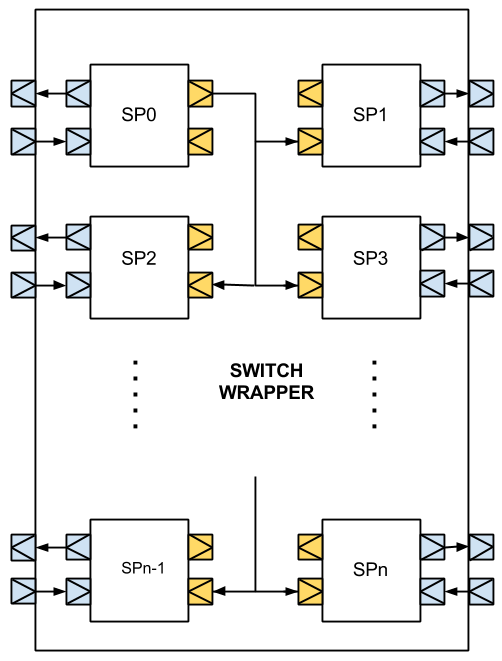
\includegraphics[scale=0.5]{switchwrapper}
             \caption{Freyja Switch Wrapper}
             \label{fig:switchwrapper}
            \end{figure}
        
        As in Fig, each switch port can send the transaction to any of the other switch port through the internal multi pass through socket. The other switch ports can receive the transaction using the multi pass through receive socket. A transaction source and destination cannot be the same operator as there is no such interconnection.
        
        \subsubsection*{Overall architecture}
            Overall architecture for 4 operators
        
         \begin{figure}[!htb]
             \centering
             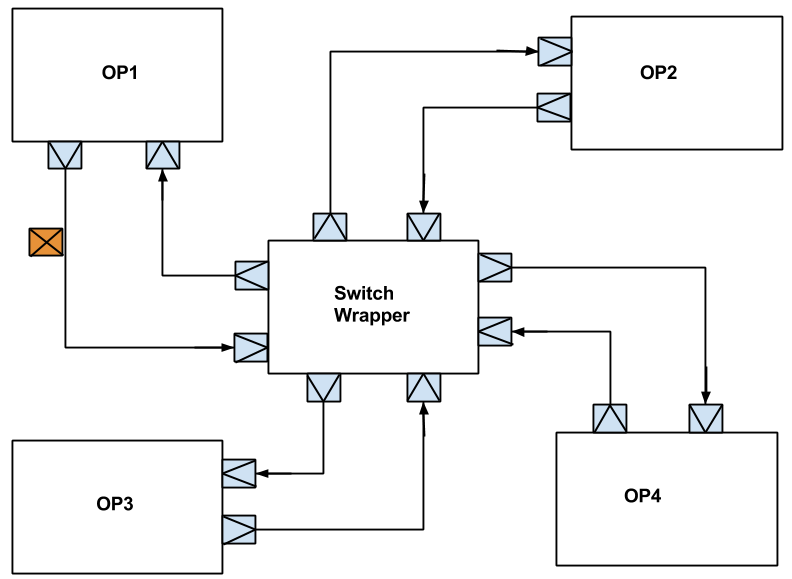
\includegraphics[scale=0.5]{Overallarchitecture}
             \caption{Freyja Architecture for 4 operators}
             \label{fig:Overallarchitecture}
            \end{figure}    
       
       As in Fig, the overall Frejya architecture consists of switch wrapper instantiating switch ports and the operator blocks for each of the operator functions. A transaction originating from operator 1 as shown in fig with Orange box can be routed to any of the other operators as destination based on the address of the payload. This address is assigned in the control block of the operator where the transaction is originated. 
       
       \clearpage
       
       \subsection{Highlevel description of the protocol}
       \clearpage
       
       \subsection{Verification and Testing}
       \clearpage
       

		\section{Developed language}
            A language description is developed to define the Freyja architecture which maps different protocol operators and their interconnections. The high level description accounts for different operator?s instantiation, transaction routing, constants in memory and error handling. Each of these is explained in detail in this chapter.
            
        \subsection{Parser implementation}
            Antlr tool is used as a parser generator to develop the language. The grammar is defined using EBNF. Antlr parser use a new parsing technology called Adaptive LL(*).This parsing strategy combines the simplicity, efficiency and predictability of conventional top-down LL(k) parser with the power of GLR like mechanism to make parsing decision. It performs the grammar analysis dynamically at runtime rather statically. The grammar analysis is moved to parse time which helps to handle any non-left recursive context free grammar.
            
            
             \begin{figure}[!htb]
                 \centering
                 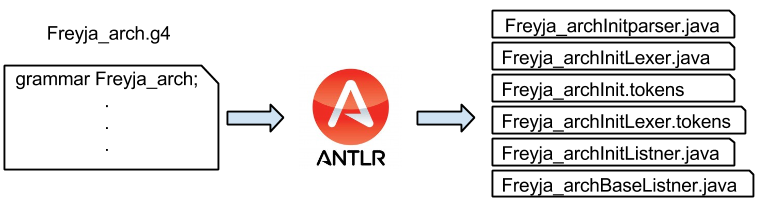
\includegraphics[scale=0.5]{antlrfiles}
                 \caption{Antlr generated Files}
                 \label{fig:antlrfiles}
                \end{figure}
        
        A brief description of the generated file are stated below:\\
        
        Freyja\_archInitparser.java: contains the parser class definition specific to grammar Freyja\_arch that recognizes our Freyja protocol processor language syntax.\\
        
        Freyja\_ArchInitLexer.java: This file contains the lexer class definition by analyzing the lexical rules in the grammar.\\
        
        Freyja\_archInit.tokens: Antlr generates a token type number to each token in the grammar and store these values in this file.\\
        
        Freyja\_ArchInitListner.java, Freyja\_archBaseListner.java: Antlr parser builds a tree walker that can trigger the callback events to a listener objects. Freyja\_archInitListner is the interface that describes the callbacks and Freyja\_ArchBaseListner is a set of empty default implementations.\\
        
        The backend functions are implemented to produce the Freyja architecture based on the language described. 
        
        
        \subsection{Operator Instantiation}
        As explained in the Fig <operator figure>, each of the operator in Freyja architecture consists of a control block to take of the transaction routing and error handling and a memory block for storing the constants and results and the process block to perform the operator function.
        
        
         \begin{figure}[!htb]
             \centering
             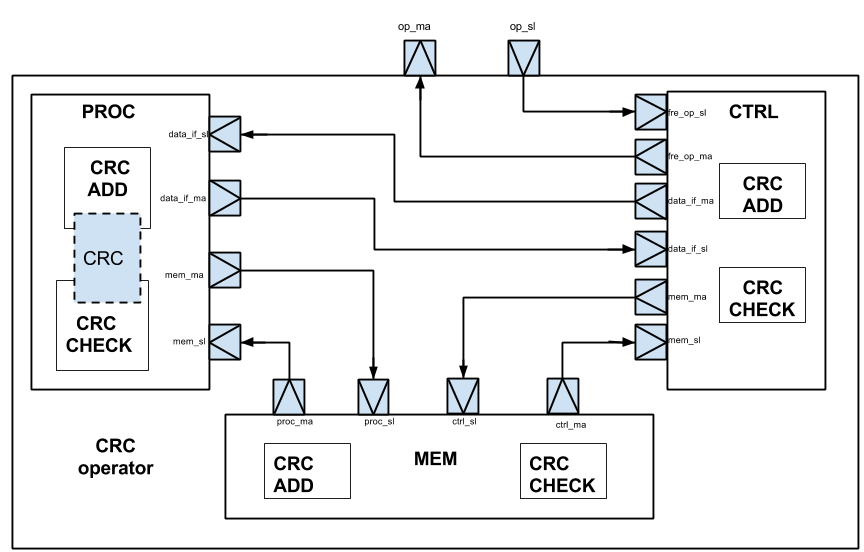
\includegraphics[scale=0.5]{CRC}
             \caption{CRC operator in Freyja Architecture}
             \label{fig:CRC}
            \end{figure}
            
            
             In a protocol processor consisting of operators for transmitting and receiving the data frames, the functions performed during the transmitting stage might need to be performed in the receiver stage. For instance, FCS is appended during the transmitting stage and in the receiver stage the computation of CRC is performed again. In addition, it performs the comparison of the received FCS value and the newly computed value to identify if the received data is erroneous or not.\\
 
            The control block of each operator has to identify the destination operator within the process block to forward the payload to exact operator. The language described has to consider this feature when instantiating the operator and defining the control blocks for each operator. An example of CRC block with CRC ADD and CRC check operators are discussed further.\\
            
            As in Fig <>, the CRC function to compute the CRC is used by both CRC ADD and CRC CHECK operators. The control block has to check if the destination operator is CRC add or CRC check and forwards the data to be processed to the correct operator and also should indicate the memory block to forward the required constants for the process blocks. This is further explained in the next section.\\
            
            The operator is defined as below:
            
            \begin{lstlisting}
            
<@\textcolor{blue}{Operator}  \textcolor{blue}{CHECKSUM}@>{
<@\textcolor{red}{sc\_name} @>: crc;
<@\textcolor{red}{op\_type} @>: crc_add,crc_check;
<@\textcolor{red}{op\_mem} @> : 0x01,0x04,0xc1,0x1d,0xb7,0x20,0x00,0x04,0x03,0x04,0x00,
           0x00,0x01,0x59,0x53,0x10,0x03,0x02,0x04;
<@\textcolor{red}{errorid} @>: 02,03;
} 
         \end{lstlisting}
        
        The operator name CHECKSUM identifies the unique operator in the Freyja architecture. The sc\_name field is used to create the systemC file with fre\_op\_ctrl\_crc,fre\_op\_proc\_crc,fre\_op\_mem\_crc files which are the control,process and memory blocks respectively. Each operator definition also takes care of including a switch port and modifying the switch wrapper functions to take care of the interconnections. 
        
        \subsection{Context switching}
        
        The context switching in the process block is performed based on the destination operator for the data packet. The interconnect information is by the control block to determine the protocol and destination operator for the data packet. The control block will then forwards the transaction to the process block where the context switching between the operators are performed. The operator type field will indicate the process block to switch between the operators.\\
        
        The control block also indicates the memory block to send the required constants for the process block. For the CRC operator, as in Fig <>, the control block will determine the protocol and the operator type and then informs the memory blocks with the transaction payload. The control block will send the received transaction to the process block. The memory block will decodes the operator and then sends the constants required for the operator through a transaction. The process block will do the context switching of operator between CRC add and CRC check to obtain the result according to the destination operator.\\ 
        
        Once the results are obtained, the process block will send it to the control block. The control block will forward the transaction to the next block.\\ 
        
      
        \subsection{Memory}
        
        The memory block is designed to store the constants required for the operators and also to store the results. But currently the results are not stored in memory, as only one protocol is implemented.\\
         
        The constants to be stored in the memory are indicated in the op\_mem field. Each operator is allowed store all the constants in the memory and based on the operator in use the constants can be forwarded to the process block through a transaction. As in operator checksum definition, the memory contains 19 bytes which are used by the CRC16 and CRC 32 operators.\\
         
        Memory transaction for each protocol are described in the language as below  
        
         \begin{lstlisting}
<@\textcolor{blue}{memory} @>{
<@\textcolor{red}{crc\_add} @>   :00 to 08;
<@\textcolor{red}{crc\_check} @> :00 to 07,09;
<@\textcolor{red}{scram} @>     :00 to 07: 
<@\textcolor{red}{descram} @>   :00 to 07;
} 
        \end{lstlisting}
       
        
        As in code above the first 8 bytes of memory contents are sent as a transaction from memory for the CRC ADD operation in CHECKSUM operator. The different forms of notation can be observed in the CRC check wherein the memory bytes can be specified with individual address. Each protocol with the memory code as above can send transaction for different operators. In the above code, the crc add,crc check,scram and descram send the transaction to their respective blocks.
        
        
        
        \subsection{Transaction handling}
        
        The transaction routing for each protocol is described in the input file using the below syntax \\
        
        CONNECT: <source operator> to <Destination operator>\\
        
        Based on these all the control blocks will be configured with the destination address for the payload. The switch interconnect will send the transaction to the next operator based on this address. This mapping defines the transaction routing for each protocols and is used to build the destination address automatically using the input description. 
        
        \subsection{Error handling}
        
        Any erroneous packets can be sent to the error handler from each of the operator. The control block will check for the process block result, if there are any errors then it informs the control block through the FBI header and the control block will send the payload to error handler for further processing and will not be sent to the destination operator.\\
        
        The error id for each operator can be implicitly assumed or even possible to mention as an explicit number. 
        
        
        
        
        
		\clearpage

		\section{Tests}
         This chapter describes the test system, testing strategy, input protocol file, discussion about output obtained.
         
         \subsection{Complete Test System}
            As in Fig <>, the first switch port is connected to the UVM test bench. The UVM environment will drive the input signals according to the Freyja architecture. The Freyja interconnect consists of 4 bytes header field and the data payload as in Fig <>. 
            In SystemC implementation the first byte is considered to hold the unique protocol id and the second byte to have the unique operator id, the third byte and fourth byte are for Flow control and Context/error handling. 
            
        
          \begin{figure}[!htb]
              \centering
              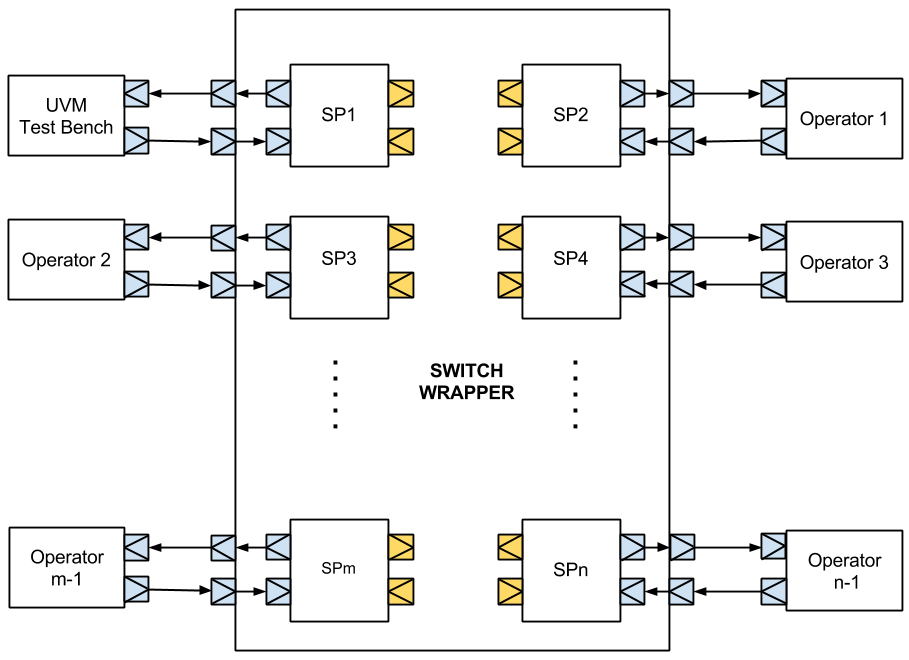
\includegraphics[scale=0.5]{testsystem}
              \caption{Complete Test System(*Multiport interconnections not shown)}
              \label{fig:testsystem}
            \end{figure}
            
            
            The data bit width is suggested to be 80bits. This complete data is randomly generated with constraints from UVM sequencer. The UVM driver will drive the input signals to the Freyja architecture.  The data is sent as a transaction payload. 
            
        
        \begin{figure}[!htb]
            \centering
            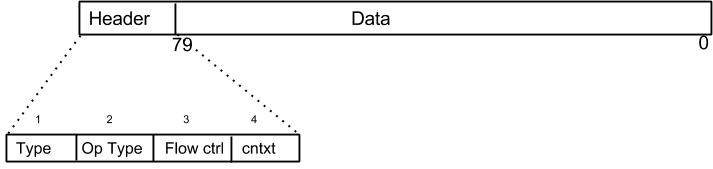
\includegraphics[scale=0.5]{header}
            \caption{FBI Interconnect}
            \label{fig:header}
        \end{figure}
        
        \subsection{Payload and blocking transport}
        
        Each generic payload transaction has a standard set of bus attributes:
        Command
        Address
        Data
        Byte enables
        Streaming width
        Response status
        The default values are set for the unused attributes. The address is initially set in the test bench and in the Freyja architecture; each operator control block will modify the address field based on the destination operator address. The data field is set to the result of the operator process blocks.
        
        
        
        
       
        
        
        \subsection{Input and output}
        
         \begin{figure}[!htb]
             \centering
             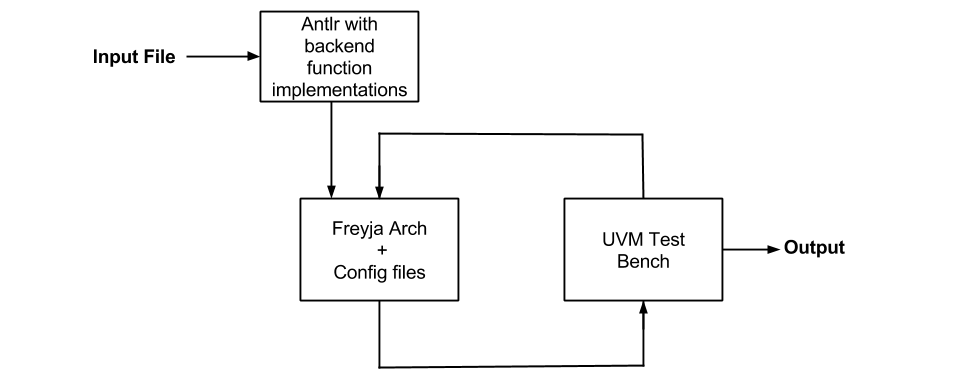
\includegraphics[scale=0.5]{inputoutput}
             \caption{Input and Output of the system}
             \label{fig:inputoutput}
            \end{figure}
        
        The input file is the description of the protocol using the language defined by the EBNF grammar. The input file is parsed by the Antlr tool; the backend functions are triggered during parsing to output the Freyja architecture and the reconfigurable files. The UVM test bench will send the transaction to the Freyja architecture. The simulation is performed using Quartus tool chain. The transaction is initiated from the UVM to the Freyja architecture and the final transaction is received back in the UVM. An example of instantiatig 4 operator blocks and interconnecting them using the input file and the corresponding output is shown below:
        
       
         \subsection{Blocking transport and timing annotation}
         The transaction is sent through the socket using the b\_transport method of the TLM\-2.0 blocking transport interface, which passes its transaction arguments by reference and has no return value. The b\_transport also carries the timing annotation which is not configured as the main interest as of now is to model the functionality of the target and not modeling any timing detail.
         
         
        
        
		\clearpage

        \section{Analysis}
            This chapter explains the analysis of the framework through the integration of Ethernet protocol into the Freyja architecture. Ethernet operators are integrated into the system of files generated from the Antlr tool. To show the context switching between different protocols, Xio-s CRC16 operator is also integrated. The first section analyses the process and results of Ethernet integration and section 6.2 explains the Xio-s protocol integration.
        
        
        \subsection{Ethernet}
        \subsection{Xio}
        \clearpage

		\section{Conclusion}
        \subsection{Limitations}
        \subsection{Future work}
		\clearpage



		\begin{filecontents*}{references.bib}


		@INPROCEEDINGS{5335678, 
			author={Szczesny, D. and Showk, A. and Hessel, S. and Bilgic, A. and Hildebrand, U. and Frascolla, V.}, 
			booktitle={System-on-Chip, 2009. SOC 2009. International Symposium on}, 
			title={Performance analysis of LTE protocol processing on an ARM based mobile platform}, 
			year={2009}, 
			month={Oct}, 
			pages={056-063}, 
			keywords={hardware-software codesign;mobile communication;mobile handsets;virtual prototyping;ARM based mobile platform;LTE protocol processing;long term evolution layer;robust header compression;Acceleration;Computational modeling;Hardware;Long Term Evolution;Mobile computing;Mobile handsets;Performance analysis;Physical layer;Protocols;Virtual prototyping}, 
			doi={10.1109/SOCC.2009.5335678},}

			@INPROCEEDINGS{558379, 
				author={Abnous, A. and Rabaey, J.}, 
				booktitle={VLSI Signal Processing, IX, 1996., [Workshop on]}, 
				title={Ultra-low-power domain-specific multimedia processors}, 
				year={1996}, 
				month={Oct}, 
				pages={461-470}, 
				keywords={computer architecture;computer networks;digital signal processing chips;integrated circuit design;land mobile radio;mobile radio;multimedia communication;portable computers;radio equipment;communication capabilities;hybrid architecture template;multimedia services;portable communication devices;portable computing;programmable devices;signal processing applications;ultra-low-power domain-specific multimedia processors;Computer aided instruction;Computer architecture;Decoding;Digital signal processing;Energy efficiency;Kernel;Multimedia computing;Portable computers;Power engineering computing;Signal processing algorithms}, 
				doi={10.1109/VLSISP.1996.558379},}

				@INPROCEEDINGS{1106752, 
					author={Keutzer, K. and Malik, S. and Newton, A.R.}, 
					booktitle={Computer Design: VLSI in Computers and Processors, 2002. Proceedings. 2002 IEEE International Conference on}, 
					title={From ASIC to ASIP: the next design discontinuity}, 
					year={2002}, 
					month={}, 
					pages={84-90}, 
					keywords={application specific integrated circuits;logic design;programmable circuits;ASIC;ASIP;Application Specific Instruction Set Processors;Application Specific Integrated Circuits;application implementation philosophy;programmable platforms;Application software;Application specific integrated circuits;Application specific processors;Computational geometry;Costs;Design methodology;Hardware;Manufacturing;Productivity;Time to market}, 
					doi={10.1109/ICCD.2002.1106752}, 
					ISSN={1063-6404},}

					@INPROCEEDINGS{6868627, 
						author={Badawi, M. and Hemani, A. and Zhonghai Lu}, 
						booktitle={Application-specific Systems, Architectures and Processors (ASAP), 2014 IEEE 25th International Conference on}, 
						title={Customizable coarse-grained energy-efficient reconfigurable packet processing architecture}, 
						year={2014}, 
						month={June}, 
						pages={30-35}, 
						keywords={application specific integrated circuits;multiprocessing systems;reconfigurable architectures;agile reconfigurability;custom ASIC implementation;customizable coarse grained energy efficient reconfigurable packet processing architecture;hardwired ASIC implementation;programmable protocol processor;real-life Voice-Over IP traffic;reconfigurable multicore packet processing architecture;retaining flexibility;time critical adaptability;Application specific integrated circuits;Delays;IP networks;Program processors;Protocols;Registers;Time factors}, 
						doi={10.1109/ASAP.2014.6868627},}

						@ARTICLE{1114865, 
							author={Estrin, G.}, 
							journal={Annals of the History of Computing, IEEE}, 
							title={Reconfigurable computer origins: the UCLA fixed-plus-variable (F+V) structure computer}, 
							year={2002}, 
							month={Oct}, 
							volume={24}, 
							number={4}, 
							pages={3-9}, 
							keywords={reconfigurable architectures;UCLA fixed-plus-variable structure computer;University of California at Los Angeles;models;reconfigurable computer architectures;reconfigurable systems analysis;reconfigurable systems design;tools;Circuits;Computer architecture;Contracts;Hardware;High performance computing;Laboratories;Mathematics;Microprocessors;System analysis and design;Telephony}, 
							doi={10.1109/MAHC.2002.1114865}, 
							ISSN={1058-6180},}

							@misc{page1985re,
								title={Re-programmable PLA},
								author={Page, D.W. and Peterson, L.V.R.},
								url={http://www.google.com/patents/US4508977},
								year={1985},
								month=apr # "~2",
								publisher={Google Patents},
								note={US Patent 4,508,977}
							}

                        @article{JACST518,
	                    author = {Abida Waza and Roohie Naaz Mir and Hakim Najeeb-ud-din},
	                    title = {Reconfigurable Architectures},
	                    journal = {Journal of Advanced Computer Science \& Technology},
                    	volume = {1},
	                    number = {4},
                    	year = {2012},
	                    keywords = {},
	                    abstract = {In the area of computer architecture, designers are faced with the trade-of between flexibility and performance. The architectural choices span a wide spectrum, with general-purpose processors and application specific integrated circuits (ASICs) at opposite ends. General-purpose processors are not optimized to specific applications; they are flexible due to their versatile instruction sets that allow the implementation of every computable task. ASICs are dedicated hardware devices that can achieve higher performance, require less silicon area, and are less power-consuming than instruction-level programmable processors. However, they lack in flexibility. Reconfigurable computer architectures promise to overcome this traditional trade-off and achieve both, the high performance of ASICs and the flexibility of general-purpose processors.},
	                    issn = {2227-4332},
	                    url = {http://www.sciencepubco.com/index.php/JACST/article/view/518},
	                    pages = {337--346}

                    	@INPROCEEDINGS{5351593, 
	                	author={Shami, M.A. and Hemani, A.}, 
	                	booktitle={ASIC, 2009. ASICON '09. IEEE 8th International Conference on}, 
		                title={Partially reconfigurable interconnection network for dynamically reprogrammable resource array}, 
		                year={2009}, 
		                month={Oct}, 
	                	pages={122-125}, 
	                	keywords={multiprocessor interconnection networks;reconfigurable architectures;binary encoding;dynamically reprogrammable resource array;innovative regular nonblocking interconnection network;low latency interconnection network;partially reconfigurable interconnection network;point-to-multipoint interconnection network;point-to-point interconnection network;sliding window connectivity;Delay;Energy efficiency;Fabrics;Multiplexing;Multiprocessor interconnection networks;Nearest neighbor searches;Parallel processing;Reconfigurable architectures;Reconfigurable logic;Signal processing algorithms;CGRA;Dynamically Reconfigurable;Interconnects;Partially Reconfigurable}, 
		                doi={10.1109/ASICON.2009.5351593},}
                    
                    
                         @comment{ Anne H�kansson, Portal of Research Methods and Methodologies for 
                             Research Projects and Degree Projects. WORLDCOMP'13 - The 2013 
                             World Congress in Computer Science, Computer Engineering, and 
                             Applied Computing, 22-25 July, 2013 Las Vegas, Nevada; USA }
                            @book{2013portal,
                                author = "Anne H�kansson",
                                title = "Portal of Research Methods and Methodologies for Research Projects and Degree Projects",
                                publisher = "WORLDCOMP'13 - The 2013 World Congress in Computer Science, Computer Engineering, and Applied Computing",
                                pages = "22--25",
                                year = 2013
                            }
                            
                           @ARTICLE{1617814, 
                               journal={IEEE Std 1666-2005}, 
                               title={IEEE Standard System C Language Reference Manual}, 
                               year={2006}, 
                               month={}, 
                               pages={0\_1-423}, 
                               doi={10.1109/IEEESTD.2006.99475},}
                            
                           @ARTICLE{4066263, 
                               author={Peterson, W.W. and Brown, D.T.}, 
                               journal={Proceedings of the IRE}, 
                               title={Cyclic Codes for Error Detection}, 
                               year={1961}, 
                               month={Jan}, 
                               volume={49}, 
                               number={1}, 
                               pages={228-235}, 
                               keywords={Binary codes;Data communication;Decoding;Encoding;Error correction codes;Feedback;Fires;Information theory;Mathematics;Polynomials}, 
                               doi={10.1109/JRPROC.1961.287814}, 
                               ISSN={0096-8390},}
                            
}


\end{filecontents*}
\bibliographystyle{ieeetr}
\bibliography{references}
\addcontentsline{toc}{section}{References}

\end{document}
